% pyformex manual --- gui
% $Id$
% (C) B.Verhegghe

\chapter{The Graphical User Interface}
\label{cha:gui}

\section{Starting the GUI}
You start the \pyf GUI by entering the command \Code{pyformex --gui}. Depending on your installation, you may also have a panel or menu button on your desktop from which you can start the \pyf graphical interface by a simple mouse click. 
%Finally, you can start the GUI with the command \Code{startGUI()} in a \pyf script.

When the main window appears, it will look like the one shown in the figure~\ref{fig:gui}. Your window manager will most likely have put some decorations around it, but these are very much OS and window manager dependent and are therefore not shown in the figure.

\begin{figure}[ht]
  \centering
  \begin{makeimage}
  \end{makeimage}
  \begin{latexonly}
    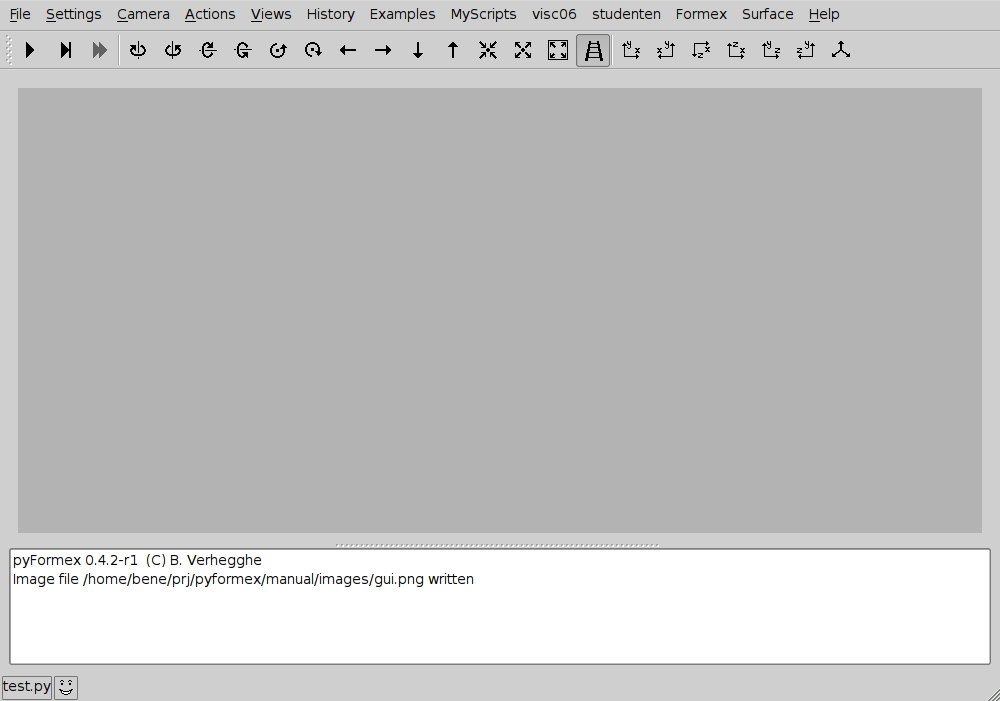
\includegraphics[width=10cm]{images/gui}
  \end{latexonly}
  \begin{htmlonly}
    \htmladdimg{../images/gui.png}
  \end{htmlonly}  
  \caption{The pyFormex main window}
  \label{fig:gui}
\end{figure}

\section{Basic use of the GUI}

As \pyf is still in its infancy, the GUI is subject to frequent changes and it would make no sense to cover here every single aspect of it. Rather we will describe the most important functions, so that users can quickly get used to working with \pyf. Also we will present some of the more obscure features that users may not expect but yet might be very useful. 

The \pyf window (figure~\ref{fig:gui}) comprises 5 parts. From top to bottom these are:
\begin{enumerate}
\item the menu bar,
\item the tool bar,
\item the canvas (empty in the figure),
\item the message board, and
\item the status bar.
\end{enumerate}

Many of these parts look and work in a rather familiar way. The menu bar gives access to most of the \pyf GUI features through a series of pull-down menus.
The most import functions are described in following sections.

The toolbar contains a series of buttons that trigger actions when clicked upon. This provides an easier access to some frequently used functions, mainly for changing the viewing parameters.

The canvas is a drawing board where your \pyf scripts can show the created geometrical structures and provide them with full 3D view and manipulation functions. This is obviously the most important part of the GUI, and even the main reason for having a GUI at all. However, the contents of the canvas is often mainly created by calling drawing functions from a script. This part of the GUI is therefore treated in full detail in a separate chapter. 

In the message board \pyf displays informative messages, requested results, possibly also errors and any text that your \pyf script writes out.

The status bar shows the current status of the GUI. For now this only contains the filename of the current script and an indicator if this file has been recognized as a \pyf script (happy face) or not (unhappy face).


Between the canvas and the message board is a splitter allowing resizing the parts of the window occupied by the canvas and message board. The mouse cursor changes to a vertical resizing symbol when you move over it. Just click on the splitter and move the mouse up or down to adjust the canvas/message board to your likings. 

The \pyf main window can be resized in the usual ways. 

   
\section{The file menu}
\label{sec:file-menu}


   
\section{The viewport menu}
\label{sec:viewport-menu}



\section{Customizing the GUI}
\label{sec:customize-gui}

Some parts of the \pyformex GUI can easily be customized by the user. 
The appearance (widget style and fonts) can be changed from the preferences menu. Custom menus can be added by executing a script. Both are very simple tasks even for beginning users. They are explained shortly hereafter.

Experienced users with a sufficient knowledge of Python and GUI building with Qt can of course use all their skills to tune every single aspect of the \pyformex GUI according to their wishes. If you send us your modifications, we might even include them in the official distribution.


\subsection{Changing the appearance of the GUI}
\label{sec:chang-appe-gui}


\subsection{Adding your scripts in a menu}
\label{sec:adding-scripts-menu}
By default, pyFormex adds all the example scripts that come with the distribution in a single menu accessible from the menubar. The scripts in this menu are executed by selecting them from the menu. This is easier than opening the file and then executing it.

You can customize this scripts menu and add your own scripts directories to it.
Just add a line like the following to the main section of your .pyformexrc configuration file:\\
\Code{scriptdirs = [('Examples', None), ('My Scripts', '/home/me/myscripts'), ('More', '/home/me/morescripts')]}

Each tuple in this list consists of a string to be used as menu title and the absolute path of a directory with your scripts. From each such directory all the files that are recognized as \pyformex scripts and do no start with a '.' or '_', will be included in the menu. If your scriptdirs setting has only one item, the menu item will be created directly in the menubar. If there are multiple items, a top menu named 'Scripts' will be created with submenus for each entry.

Notice the special entry for the examples supplied with the distribution. You do not specify the directory where the examples are: you would probably not even know the correct path, and it could change when a new version of \pyf is installed. As long as you keep its name to 'Examples' (in any case: 'examples' would work as well) and the path set to None (unquoted!), \pyformex will itself try to detect the path to the installed examples. 


\subsection{Adding custom menus}
\label{sec:adding-custom-menus}

When you start using \pyformex for serious work, you will probably run into complex scripts built from simpler subtasks that are not necessarily always executed in the same order. While the \pyformex scripting language offers enough functions to ask the user which parts of the script should be executed, in some cases it might be better to extend the \pyformex GUI with custom menus to execute some parts of your script.

For this purpose, the gui.widgets module of \pyformex provides a Menu widget class. Its use is illustrated in the example Stl.py.

%%% Local Variables: 
%%% mode: latex
%%% TeX-master: "manual"
%%% End: 
